\appendix

\chapter{Reproducibility}
\label{appendix:simulationParams}

The full simulation code as well as the Jupyter Notebooks for post-processing are uploaded to the
GitLab repository \cite{tobiaStudentRepo} under the PSI domain.
The structure of the repository is detailed in the top-level \texttt{README.md} file.
If the contents of a directory are not self-explanatory we also add a \texttt{README.md} with
further information.

For running the simulation we provide Bash scripts where simulation parameters can be set.
A summary of the simulation code and how to run it can be found in the following slides
\texttt{presentations/handover/main.pdf}.
The data used for generating the plots in this report are stored in the compressed file
\texttt{compressed\_data.zip} due to its size.
The directory structure therein mirrors the one found in the repository.
The decompressed files can then be copied over to the respective directory containing a Jupyter
Notebook.

\subsubsection{Simulation Parameters}

We use partially normalized units in our Langevin solver where it makes sense (Table
\ref{table:langevinUnits}).

\begin{table}[h]
    \caption{Unit convention used in the Langevin solver.}
    \label{table:langevinUnits}
    \begin{center}
        \begin{tabular}[c]{llll}
            \toprule
            \multicolumn{1}{l}{\textbf{Type}} & 
            \multicolumn{1}{l}{\textbf{Symbol}} & 
            \multicolumn{1}{l}{\textbf{Unit value}} &
            \multicolumn{1}{l}{\textbf{Normalizing Constant}} \\
            \hline
            Length & [L] & $10^{-2}\ \text{m}$ & -\\
            Time & [T] & $1\ \text{s}$ & - \\
            Mass & [M] & $9.109\times10^{-31}\ \text{kg}$ & $m_e$ \\
            Charge & [Q] & $1.602\times10^{-19}\ \text{C}$ & $q_e$ \\
            \hline
        \end{tabular}
    \end{center}
\end{table}

Subsequently, we list the parameters and units used in the Langevin solver (Table
\ref{table:langevinDefaultParams}) and the reference \gls{p3m} implementation by Ulmer \cite{p3m_ulmer} (Table
\ref{table:UlmerDefaultParams}).

\pagebreak

\section{Parameters of the Langevin solver}
\label{appendix:ourParams}

\begin{table}[h]
    \caption{Default parameters of the Langevin Solver.}
    \label{table:langevinDefaultParams}
    \begin{center}
        \begin{tabular}[c]{llll}
            \toprule
            \multicolumn{1}{l}{\textbf{Parameter}} & 
            \multicolumn{1}{l}{\textbf{Description}} & 
            \multicolumn{1}{l}{\textbf{Default value}} &
            \multicolumn{1}{l}{\textbf{Unit}} \\
            \hline
            $r_{beam}$ & Beam radius & 0.001774  & [L] \\
            $L_{box}$ & Box length & 0.01 & [L] \\
            $N_p$ & Number of Macroparticles & 156055 & - \\
            $N_r$ & Spatial grid points per dimension & 256 & - \\
            $dt$ & Time step size & $2.15623\times10^{-13}$ & [T] \\
            $N_t$ & Number of time steps & 1000 & - \\
            $q_e$ & Particle charge (normalized) & -1.0 & [Q] \\
            $m_e$ & Particle mass (normalized) & 1.0 & [M] \\
            $f_c$ & Focusing strength & 1.5 & - \\
            $\epsilon^{-1}$ & Inverse vacuum permittivity & $3.182609\times10^9$ & $\frac{\text{[L]}^3
            \text{[M]}}{\text{[T]}^2 \text{[Q]}^2}$ \\
                $\Gamma$ & Prefactor Rosenbluth potentials & $8.0604\times10^{18}$ &
                $\text{[L]}^6/\text{[T]}^4$  \\
            $N_v$ & Velocity grid points per dimension & 64 & - \\
            $v_{max}$ & Maximum extent of each velocity quadrant & $5.0\times10^7$ & [L]/[T] \\

            \hline
        \end{tabular}
    \end{center}
\end{table}

\section{Parameters of the \gls{p3m} Reference Implementation}
\label{appendix:ulmerParams}

\begin{table}[h]
    \caption{Default parameters of the \gls{dih} solver by Ulmer.}
    \label{table:UlmerDefaultParams}
    \begin{center}
        \begin{tabular}[c]{llll}
            \toprule
            \multicolumn{1}{l}{\textbf{Parameter}} & 
            \multicolumn{1}{l}{\textbf{Description}} & 
            \multicolumn{1}{l}{\textbf{Default value}} &
            \multicolumn{1}{l}{\textbf{Unit}} \\
            \hline
            $r_{beam}$ & Beam radius & 0.001774  & [L] \\
            $L_{box}$ & Box length & 0.01 & [L] \\
            $N_p$ & Number of Macroparticles & 156055 & - \\
            $N_r$ & Spatial grid points per dimension & 256 & - \\
            $dt$ & Time step size & $2.15623\times10^{-13}$ & [T] \\
            $N_t$ & Number of time steps & 1000 & - \\
            $q_e$ & Particle charge (normalized) & -1.0 & - \\
            $m_e$ & Particle mass (normalized) & 1.0 & - \\
            $f_c$ & Focusing strength & 1.5 & - \\
            $r_c$ & Cut-off radius for \gls{pp} interactions & $3.125\times10^{-4}$ & [L] \\
            $\varepsilon$ & regularization for \gls{pp} interactions & 0 & [L] \\
            $\alpha$ & Green's function splitting parameter & $1.0\times10^6$ & - \\
            \hline
        \end{tabular}
    \end{center}
\end{table}


\clearpage
\chapter{Convergence Study}
\label{appendix:convergenceStudy}

\section{Gaussian Testcase}

\begin{figure}[h]
  \begin{subfigure}[b]{0.50\textwidth}
    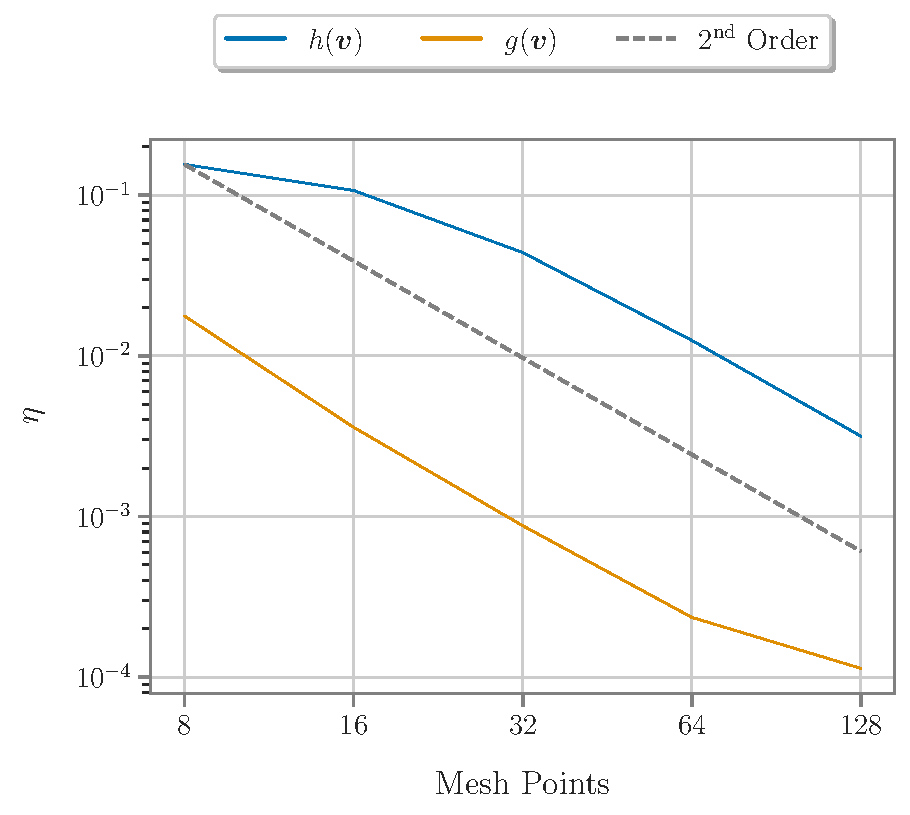
\includegraphics[width=\textwidth]{figures/appendix/convergenceStudy/hg_005vmax_HOCKNEY.pdf}
    \caption{}
    \label{fig:convergence_hg_HOCKNEY}
  \end{subfigure}
  \hfill
  \begin{subfigure}[b]{0.50\textwidth}
    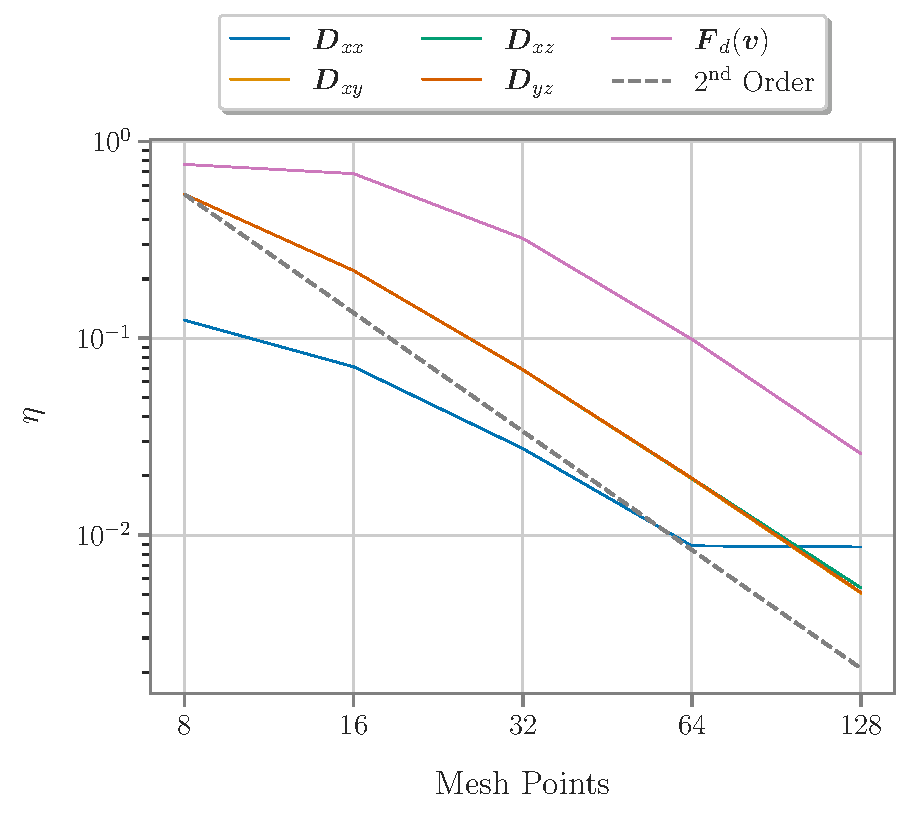
\includegraphics[width=\textwidth]{figures/appendix/convergenceStudy/D+Fd_005vmax_HOCKNEY.pdf}
    \caption{}
    \label{fig:convergence_DFd_HOCKNEY}
  \end{subfigure}
  \caption{Convergence study of Rosenbluth potentials (\ref{fig:convergence_hg_HOCKNEY}) solved with Hockney's
      algorithm and their corresponding collisional coefficients (\ref{fig:convergence_DFd_HOCKNEY}) for a 
  Gaussian velocity distribution following the same statistics as apparent in the \gls{dih} problem.}
\end{figure}

\begin{figure}
    \begin{center}
        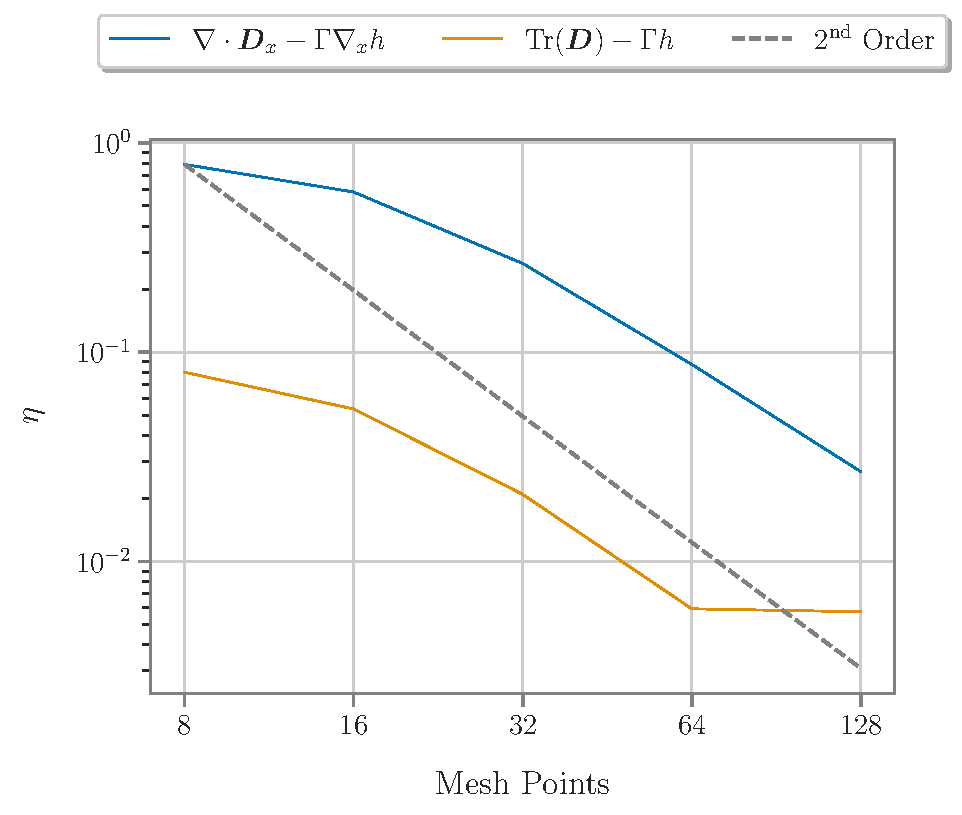
\includegraphics[width=0.62\textwidth]{figures/appendix/convergenceStudy/identities_convergence_sigma005vmax_HOCKNEY.pdf}
    \end{center}
    \caption{Convergence study of the identities defined in Equation \ref{eq:rb_identities}.}
    \label{fig:meshsize_test_HOCKNEY}
\end{figure}

\clearpage
\chapter{\gls{ldlt} Decomposition}
\label{appendix:LDLT}

For our Langevin formulation of the Vlasov-Poisson-Fokker-Planck equation we need to factorize the
3x3 diffusion matrices $\matr D$ with a Cholesky decomposition.
Due to aforementioned reasons (see Section \ref{section:rb_discretization}), this is most efficiently
achieved with a \gls{ldlt} decomposition.
Our implementation is a straighforward unrolled implementation of this recursive algorithm.
In the following listing of the implementation we state invariants (IPPL macros) that require the matrix to be
semi-positive definite ($\texttt{D} \ge 0$ on line 24).

\begin{listing}[!ht]
    \vspace{3.3mm}
    \inputminted[]{c++}{code_snippets/LDLT.cpp}
    \caption{C++ function computing $\matr Q$ from a given 3x3 matrix via the \gls{ldlt} decomposition.}
\label{listing:LDLTcode}
\end{listing}

\clearpage
\chapter{Supplementary Material of the \gls{dih} Experiments}
\label{appendix:suppDIH}

\begin{figure}[!ht]
    \begin{center}
        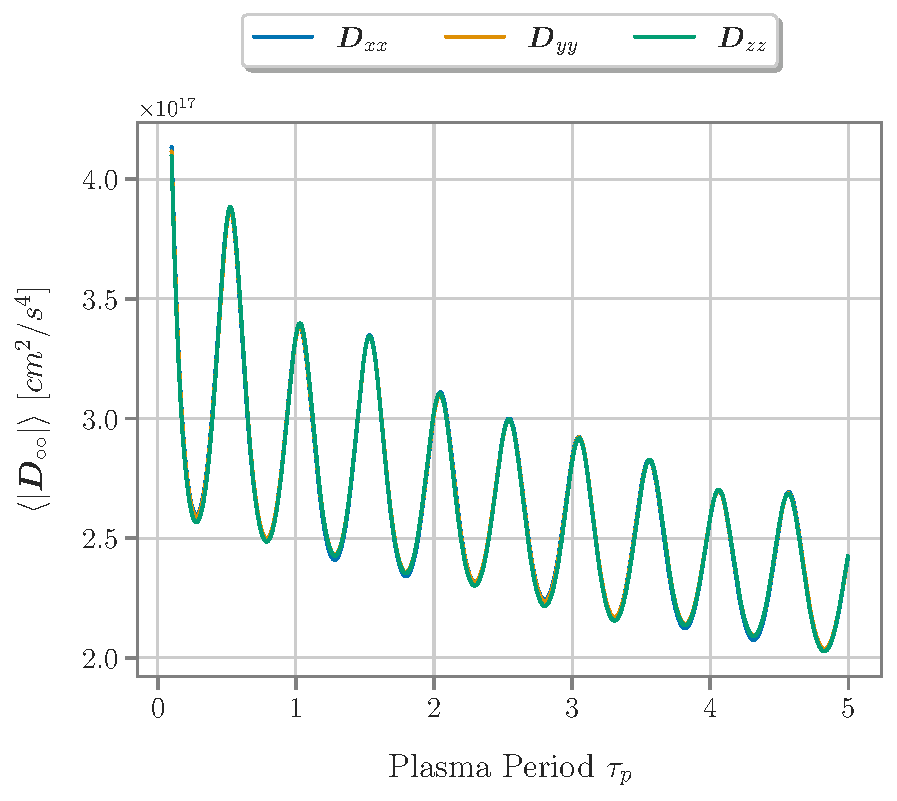
\includegraphics[width=0.62\textwidth]{figures/appendix/DIH_experiments/D_avg_diag.pdf}
    \end{center}
    \caption{Average absolute value of the diagonal diffusion coefficients over 5 plasma periods.}
    \label{fig:Ddiag_avg}
\end{figure}

\begin{figure}[!ht]
    \begin{center}
        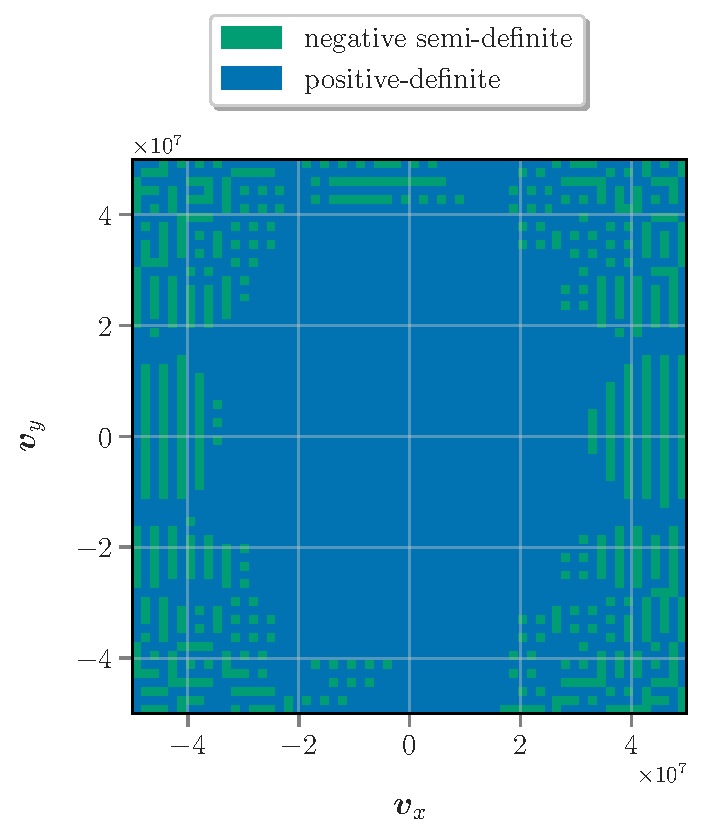
\includegraphics[width=0.47\textwidth]{figures/appendix/DIH_experiments/D_cholesky_it0800_spectralHess.pdf}
    \end{center}
    \caption{Slice through the diffusion matrix field computed with the Hessian operator with
        spectral accuracy at $\vect v_z = 0$ and $t = 4 \tau_p$ indicating the 
        matrix property for each entry.}
    \label{fig:D_cholesky_spectralHess}
\end{figure}

\clearpage
\chapter{Chainable Differential Operators}
\label{appendix:chainable_operators}

Efficient and versatile stencil operators are at the heart of many numerical simulation codes.
Thus, it does not come as a surprise that there exist a wealth of stencil libraries for almost any
existing computer language (i.e. \cite{dahm2021gt4py}, \cite{stencilStream} or \cite{bianco2012generic}).

For our work we relied on a \gls{fd} implementation of a Hessian operator (Eq.
\ref{eq:diffHess}) in \gls{ippl}
\cite{adelmann2019opal} for the diffusion coefficient computation.
It implements a compact $2^{\text{nd}}$ order centered stencil. Unfortunately this comes with the
drawback that the computed Hessian matrices along either system boundary cannot provide an accurate
result, as they access values at the ghost-cells that have no physical meaning (due to our decision to 
model the velocity space with open boundary conditions). 
We want to create a flexible interface for defining differential
operators by a combination of \gls{fd} stencils (i.e. forward-, backward difference) which avoids
code duplication as much as possible.

A differential operator can consist of one or multiple mathematically chained operators. We define a multi-index $\alpha = (\alpha_1, \alpha_2, \cdots,
\alpha_n)$ and its cardinality as $\lvert \alpha \rvert = \sum_{i=1}^n \alpha_i$, such that we are able
to express a chained operator

\begin{equation}
    \mathcal G^{\alpha} = \frac{\partial^{\lvert \alpha \rvert}}{\partial
    x_1^{\alpha_1} \partial x_2^{\alpha_2} \cdots \partial x_n^{\alpha_n}}.
    \label{eq:chainedOperator}
\end{equation}

For simplicity we set $n=3$, as all our simulations are carried out in 3 dimensions and set the
requirement that the user can choose a specific stencil type for either dimension.

As an example we would like to create a $2^{\text{nd}}$ order accurate operator for the first
derivative that does not access values outside the system boundaries on the lower $x$-axis.
A potential candidate stencil defining a 1D forward \gls{fd} scheme looks as follows:
\begin{equation}
    \frac{\partial}{\partial x}f(x_k) = \frac{-3 x_{k-1} + 4 x_{k} - 2 x_{k+1}}{2h_x}.
    \label{eq:forwardStencil}
\end{equation}
Template metaprogramming provides us with a powerful tool to construct and chain such operators at
compile time. At run time the user can then apply the operator to a certain index of the field of
interest to emulate his custom differential operator.

We continue to give the reader an insight into how we implemented this. For brevity, we
omit some details regarding base classes and utility functions. The full code is available on
\cite{tobiaStudentRepo}.
The 1D stencil of Eq. \ref{eq:forwardStencil} is implemented in C++ as shown in Listing \ref{listing:enums}. 

\begin{listing}[!ht]
    \vspace{3.3mm}
    \inputminted[]{c++}{code_snippets/diffOperator/enums.cpp}
    \caption{Generic first order centered \gls{fd} stencil in 1D.}
\label{listing:enums}
\end{listing}

This or other stencils can then be encapsulated as an operator which either calls a field at a certain index
\mintinline{c++}{(i,j,k)} or another \mintinline{c++}{Callable} (i.e. a subsequent operator, exhibiting the same
signature). This behavior is exemplified in Listing \ref{listing:chainableOperators}.

\begin{listing}[!ht]
    \vspace{3.3mm}
    \inputminted[]{c++}{code_snippets/diffOperator/stencils.cpp}
    \caption{Stencil operator calling a specific stencil of type \mintinline{c++}{enum
DiffType Diff} along \mintinline{c++}{OpDim D}.}
\label{listing:chainableOperators}
\end{listing}

Following this idea, it is a straightforward endeavor to construct more sophisticated operators that
are based on multiple such chained constructs.
A simple pseudo-code example computing $\frac{\partial^2}{\partial x \partial y} f(x,y)$ in 2
dimensions is shown in Listing \ref{listing:exampleChainedOperator}.
We conclude our excursion by constructing a Hessian operator given our
stencil formulation, hence allowing the user to choose individual stencils along either dimension.
In Figure \ref{fig:customHessian_convergence} we show that this operator exhibits the correct order
of convergence (averaged over all matrix entries) for a selection of implemented stencils.

\begin{listing}[!ht]
    \vspace{3.3mm}
    \inputminted[]{c++}{code_snippets/diffOperator/chainableOperator.cpp}
    \caption{Pseudo-code for a chained operator (equivalent to $\frac{\partial^2}{\partial x
    \partial y} f(x,y)$).}
\label{listing:exampleChainedOperator}
\end{listing}

\begin{figure}
    \begin{center}
        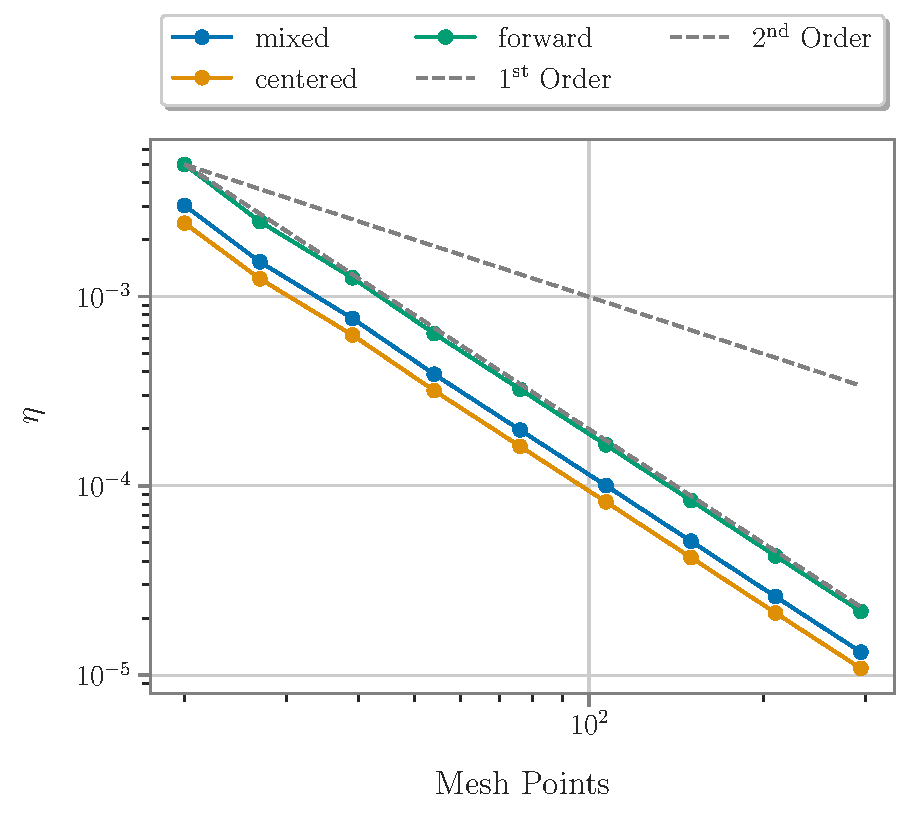
\includegraphics[width=0.62\textwidth]{figures/appendix/chainableOperator/customHessian_convergence.pdf}
    \end{center}
    \caption{Convergence study of our versatile Hessian operator. $\texttt{mixed}$
    signifies an operator which applies centered difference along the $x$-, forward
difference along $y$- and backward difference along the $z$-dimension.}
    \label{fig:customHessian_convergence}
\end{figure}



















